%Objectives : 
%\begin{itemize}
%    \item Present the rising velocity Vs. phi to demonstrate the relation with $\phi^{1/3}$ \citep{loisy2017buoyancy}
%    \item Discus the common points and differences with bubbles and solid particles. 
%    \item Present a proper definition of the drag force terms such as in \citet{wang2021numerical}. 
%    \item Discus the possible correlation between the shape /arrangement of the particles/flow lines with the rising velocity. \tb{Je ne sais pas trop quoi dire la dessus}
%    \item Show that \citet{rusche2000effect}'s fit for the drag force is not adapted for our case and propose a new one
%    \item All the references for teh Drag force terms are in \citet[chap 8]{morel2015mathematical} or in \citet{ishii2010thermo}
%\end{itemize}
%\todo[inline]{include fits of bubbly flow}

\subsection{Terminal velocity of an isolated spherical drop}
%First of all we want to investigate the dependency of the drift velocity with the volume fraction $\phi$. 
%It is known from several studies on the litterature, especially in \citep[chapter 8]{morel2015mathematical} and \citet[chapter 12]{ishii2010thermo} the the viscosity model for various system can be written generally, as,
%\begin{equation*}
%    \frac{\mu_m}{\mu_c}
%    = \left(
%        1 - \frac{\phi}{\phi_\text{max}}
%    \right)^{-2.5 \phi_\text{max}\mu_\text{eq}}
%\end{equation*}  
%with, $\mu_\text{eq} = \frac{\mu_d + 0.4 \mu_c}{\mu_d+\mu_c}$ and $\phi_\text{max}$ being the volume fraction corresponding to the \textit{maximum packing}. 
%\JL{la viscosite d'une suspension n'a rien a voir avec sa vitesse de chute meme si cela semble etre un argument donne dans la litterature... j'ai enleve tout cela pr l'instant}

In this part, we briefly review the various formulas used to calculate the drag force on a spherical droplet embedded in a steady uniform flow. As demonstrated in Appendix \ref{app:shape} the droplet remains approximatively spherical. This assumption remains valid for the whole range of parameters investigated even in high inertial regime where the maximum deviation from the spherical shape is around $10$ \%. Theoretical predictions for the force on a spherical droplet embedded in a steady uniform flow are limited to the limit of very small and very high Reynolds numbers. We define the drag coefficient, denoted as $C_D$ by the equation $F = \pi / 8 C_D \rho U_0^2 d^2$, where $F$ is the force on the drop, $U_0$ is the imposed velocity. The drag coefficient is a function of the Reynolds number $Re = \rho U_0 d /\mu $ and of is the viscosity ratio$\lambda = \mu _d /\mu _c$. % is the  as $F = C_D$ 
In the Stokes regime ($Re=0$)the drag coeficient is given by the Hadamard-Ribczynski formula


%In this section, we briefly survey the diverse formulas applied to calculate the drag force acting on a spherical droplet within a steady, uniform flow. As corroborated in Appendix \ref{app:shape}, the droplet maintains an approximate spherical shape, a validity sustained across the entire spectrum of investigated parameters, even in the high inertial regime. Theoretical predictions for the force acting on a spherical droplet in a steady uniform flow are confined to scenarios of extremely low and exceptionally high Reynolds numbers.

%We define the drag coefficient, denoted as $C_D$, by the equation F=π8CDρU02d2F = \frac{\pi}{8} C_D \rho U_0^2 d^2F=8π​CD​ρU02​d2, where FFF signifies the force on the droplet, and U0U_0U0​ is the imposed velocity. This coefficient varies with the Reynolds number Re=ρU0dμRe = \frac{\rho U_0 d}{\mu}Re=μρU0​d​ and the viscosity ratio λ=μdμc\lambda = \frac{\mu_d}{\mu_c}λ=μc​μd​​. In the Stokes regime, the drag coefficient adheres to the Hadamard-Ribczynski formula.

%In the Stokes flow regime, the drag coefficient defined as $F = $

%drag force on a spherical drop embedded in a steady uniform flow is given by the Hadamard-Ribczynski formula
%\JL{il faut choisir ton echelle caractersitique de longueur. Soit $a$ le rayon soit le diametre des particules.}
%\begin{equation}
%F_0 = -\pi \mu d U \frac{2+3\lambda}{1+\lambda}
%\end{equation}

\begin{equation}
C_D = \frac{8}{Re} \left( \frac{2+3\lambda}{1+\lambda} \right)
\end{equation}
%\ref{fig:U} shows the drift velocity $U$ divided by the stokes rising velocity of a spherical droplet $U_\text{stokes}$ defined in our notation as \citep{kim2013microhydrodynamics}, 
Balancing the drag force obtained using the previous formula with the buoyancy force one obtained the settling velocity in the Stokes regime
\begin{equation}
    U_0
    = (\rho_c - \rho_d)\frac{g d^2}{6\mu_c}\left(\frac{1+\lambda}{2 + 3\lambda}\right).
\end{equation}
In the opposite regime of very high Reynolds numbers ($Re\gg 1$), the flow outside the droplet can be considered as potential except in a thin boundary layer developping on the bubble surface. \citet{harper1968} have shown that the drag coefficient on a spherical drop is given by 

\begin{equation}
C_D = \frac{48}{Re}\left(1 + \frac{3\lambda}{2}\right)
\end{equation}
which tends toward Levich approximation in the limit of very low viscosity ratio. where higher order terms can be found in the original publication of \citet{harper1968}. A detailed investigation perfomed by Dandy et Leal have shown that the oroginal formulation by Harper and mmore became accurate for $Re\geq 200$. The above review show that in the intermediate Reynolds number regimes of the pressent study $ 1 \leq $

%to leading order as $Re = \rho U_0 d /\mu$ 


In practice the above formula are very limited randge of validity and empirical formulation have to be used for intermediate Reynolds numbers. Prendre la correlation de Rykind et Ryskin



\subsection{Hindered settling velocity}
As an exemple for a suspenison of homogeneous solid spherical particle $\phi_\text{max} = 0.62$ and for deformable particles system it can be approximated to $\phi_\text{max} = 1$. 
From this consideration we can deduce that the drift velocity $U$ is related to the volume fraction with, 
\begin{equation*}
    \frac{U(\phi)}{U_\text{stokes}} = \left\{\begin{tabular}{cc}
        $(1-\phi)^{1.5}$   & bubbles in liquid \\
        $(1-\phi)^{2.25}$   & drops in liquid \\
        $(1-\phi)^{3}$   & drops in gas \\
    \end{tabular}\right.
\end{equation*} 
Additionally, \citet{bunner2003effect} propose a scaling of $\sim (1 - \phi^{1/3})$ for spherical bubbles.
While \citet{ishii1979drag} proposed a $\sim (1 - \phi)^3$ for deformable bubbles. 

In our case, i.e. quasi spherical droplets, we reach a $\sim (1 - \phi^{1/3})$ scaling for $\lambda = 10$ and approximately a $\sim (1 - \phi^{1/2})$ scalings for $\lambda = 1$ .
\begin{figure}[h!]
    \centering
    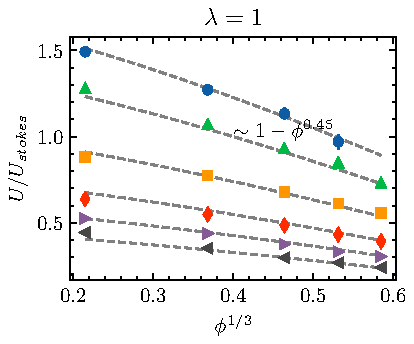
\includegraphics[height = 0.35\textwidth]{image/HOMOGENEOUS/fCA/UstokesGa_mu_r_1-0.pdf}
    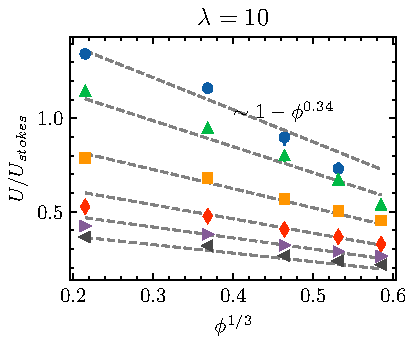
\includegraphics[height = 0.35\textwidth]{image/HOMOGENEOUS/fCA/UstokesGa_mu_r_0-1.pdf}
    \caption{Rising velocity divided by the rising velocity of an equivalent spherical drop in Stokes regime.($\bullet$) $Ga = 5$, ($\blacktriangle$) $Ga = 10$, ($\blacksquare$) $Ga = 25$ , ($\blacklozenge$) $Ga = 50$, ($\blacktriangleright$) $Ga = 75$ and ($\blacktriangleleft$) $Ga = 100$ . 
    The dashed lines are the empirical funtions (left)  
    $U/U_\text{stokes} = 2.72(Ga^{-2.77} - Ga\;10^{-3}) (1 - \phi^{0.45})$
    (right)  $U/U_\text{stokes} = 2.74(Ga^{-2.85} - Ga \;10^{-3}) (1 - \phi^{0.34})$ }
    \label{fig:U}
\end{figure}

The case for which $\lambda = 1$ have a tendency to processes more deformation, as caracterised by their averaged aspect ratio $\chi$ slightly higher than those for which $\lambda = 10$. 
The differences in the volume fraction dependency can be partially explain by this fact. 
Indeed, a  $\sim (1 - \phi^{2/3})$ power law were observed for slightly deformable bubbly flow \cite{zhang2021direct}. 
Thus it is not surprising that at low but finite deformation we found a scalings between $1/3$ and $2/3$. 

A last interesting fact is that at low $Ga$ and $\phi$ we observe a rising velocity $U / U_\text{stokes} > 1$ meaning that the rising velocity is higher than in the stokes isolated case. 
This phenomena has already been observe in \citet{loisy2017buoyancy}. 
This fact was explained to be due to the cumulative effect of the wakes in orderred array of bubbles  which tends to increases their colective velocity. 
Anyhow, since the the limit $Ga \rightarrow 0$ and $\phi \rightarrow 0$ we must recover $U/U_\text{stokes} = 1$ we can be sure that the $\phi$ scaling won't behaves like so.
Therefore it is crucial to point out that these scalings are surely not valid in the limit  $Ga \rightarrow 0$ and $\phi \rightarrow 0$ .

%\subsection{Interphase drag force}




Now we present our results for the drag force term in terms of the Reynolds number. 
\begin{figure}[h!]
    \centering
    
    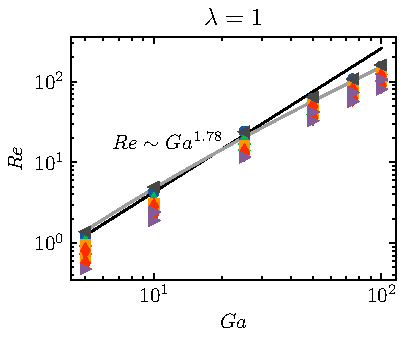
\includegraphics[height = 0.35\textwidth]{image/HOMOGENEOUS/fCA/Re_mu_r_1-0.pdf}
    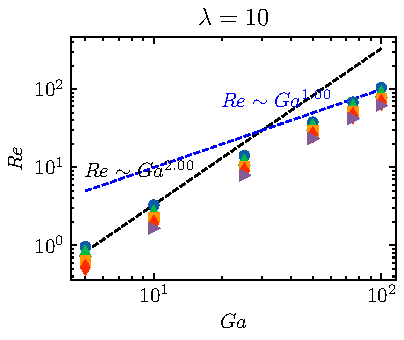
\includegraphics[height = 0.35\textwidth]{image/HOMOGENEOUS/fCA/Re_mu_r_0-1.pdf}
    
    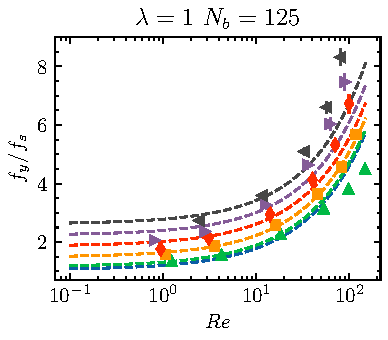
\includegraphics[height = 0.35\textwidth]{image/HOMOGENEOUS/fCA/Fstokes_N_5_l_1.pdf}
    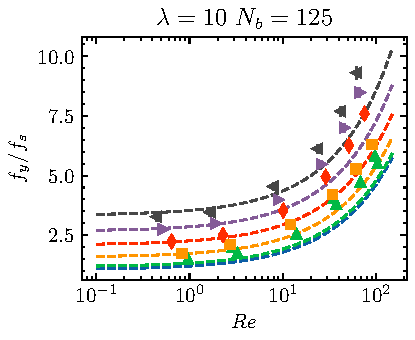
\includegraphics[height = 0.35\textwidth]{image/HOMOGENEOUS/fCA/Fstokes_N_5_l_10.pdf}
    \caption{
        (middle) Reynolds number based on the averaged rising velocity.
    (bottom) Ensemble averaged drag force divided by the stokes drag force on spherical droplet of equivalent size.
    The symbols correspond to different volume fraction ($\bullet$) $\phi = 1\%$, ($\blacktriangle$) $\phi = 5\%$, ($\blacksquare$) $\phi = 10\%$, ($\blacklozenge$) $\phi = 15\%$ and ($\blacktriangleright$) $\phi = 20\%$.
    (dashed lines) empirical formulas : extrapolation of  \citet{tenneti2011drag} for solid particles. }
    \label{fig:drag_force}
\end{figure}
\tb{As discussed in previous study that
for spherical bubbles, as the gas fraction increases and the in-
teractions become more important, the bubbles tend to align
themselves in horizontal pairs, whose average rising velocity
is lower than that of an isolated bubbl}

The interphase drag forces applied on the droplets is the buoyancy force $(\rho_d-\rho_c)v_\alpha \textbf{g}$.
The relevant quantity is therefore the dimensionless drag force, that is what is presented in the following \ref{fig:drag_force}. 


In the stokes regime the drag force on a spherical droplet is, 
\begin{equation*}
    \textbf{F}_s
    =\pi \mu_f d (\textbf{u}_p - \textbf{u}_c) \left(\frac{2+3\lambda}{1+\lambda}\right)
\end{equation*}
Let the dimensionless drag force be a function of $\lambda$ $Re$ and $\phi$, expressed such that, 
\begin{equation}
    \textbf{f}_p(Re,\phi,\lambda)
    = 
    f_1^*(Re)
    f_2^*(\phi)
    \textbf{f}_s(\lambda)
\end{equation}
where $f_{1,2}$ are coefficient which limit tends to $1$ at low $\phi$ and low $Re$. 
To determine the $\phi$ dependency we base our study on the following analysis. 
In \cite[chapter 4]{ashgriz2011handbook} they stipulate that the last droplets empirical fit was made in the study of \citet{rusche2000effect} where they performed empirical fits on experimental datas of emulsion. 
Some of which concerned droplets' sedimentation, were they stipulate that, 
\begin{align*}
    f_1^*(\phi) 
    &=1  + C_1 Re^{C_2}\\
    f_2^*(\phi) 
    &= e^{\phi K_1} + \phi K_2
    \label{eq:drag_fit}
\end{align*}
Nevertheless, the coefficients for the droplets doesn't agree with our numerical calculation. 
Instead we remark that the solid particles fit from \citet{rusche2000effect} well fits our results at $\lambda = 1$. 
Therefore, we propose to keep the shape of teh fits and adjuste our coefficient. 

\tb{Dans cette partie je ne sais pas trop quoi faire pour avoir un bon point de départ pour cree une formule empirique, je manque d'idée, notament pour ce qui est de la dépendence en $\lambda$ et pour l'explication physique des tendence observe. }
